\documentclass[12pt,a4paper]{article}

% ─── Page Layout ───────────────────────────────────────────────────────────────
\usepackage[a4paper, margin=0.8in, headheight=14pt]{geometry}

% ─── Fonts (XeLaTeX) ───────────────────────────────────────────────────────────
\usepackage{fontspec}
\usepackage{unicode-math}
\setmainfont{TeX Gyre Pagella}
\setmonofont[Scale=0.88]{TeX Gyre Cursor}
\setmathfont{Latin Modern Math}

% ─── Packages ──────────────────────────────────────────────────────────────────
\usepackage{xcolor}
\usepackage{colortbl}
\usepackage{titlesec}
\usepackage{enumitem}
\usepackage{tabularx}
\usepackage{booktabs}
\usepackage{array}
\usepackage{amsmath}
\usepackage{tikz}
\usetikzlibrary{shapes.geometric, arrows.meta, positioning, calc, fit, decorations.pathreplacing}
\usepackage{tcolorbox}
\tcbuselibrary{skins, breakable}
\usepackage{hyperref}
\usepackage{fancyhdr}
\usepackage{graphicx}
\usepackage{microtype}
\hyphenpenalty=10000
\exhyphenpenalty=10000
\sloppy
\usepackage{caption}
\usepackage{setspace}
\usepackage{multirow}
\usepackage{tocloft}

% ─── Q&A helper ────────────────────────────────────────────────────────────────
\newcommand{\Q}[1]{\textbf{#1}\par\noindent\ignorespaces}

% ─── Colour Palette ────────────────────────────────────────────────────────────
\definecolor{myred}{RGB}{196,30,58}
\definecolor{mydark}{RGB}{30,30,50}
\definecolor{mygreen}{RGB}{14,120,80}
\definecolor{myteal}{RGB}{0,130,140}
\definecolor{myamber}{RGB}{180,100,0}
\definecolor{mypurple}{RGB}{100,30,160}
\definecolor{mygray}{RGB}{246,247,249}
\definecolor{mgframe}{RGB}{180,185,200}
\definecolor{watermark}{RGB}{145,150,170}
\definecolor{hdrred}{RGB}{250,232,235}
\definecolor{hdrgreen}{RGB}{220,244,233}
\definecolor{hdrteal}{RGB}{220,242,244}
\definecolor{hdramber}{RGB}{253,242,215}
\definecolor{hdrpurple}{RGB}{238,228,255}
\definecolor{hdrgray}{RGB}{238,240,245}
\definecolor{rowalt}{RGB}{250,251,253}

% ─── Section Formatting ────────────────────────────────────────────────────────
\titleformat{\section}
  {\large\bfseries\color{myred}}{\thesection.}{0.5em}{}
  [\vspace{1pt}{\color{myred}\rule{\linewidth}{0.8pt}}]
\titleformat{\subsection}
  {\normalsize\bfseries\color{myteal}}{\thesubsection}{0.5em}{}
\titlespacing*{\section}{0pt}{18pt}{7pt}
\titlespacing*{\subsection}{0pt}{11pt}{4pt}

% ─── Paragraph ─────────────────────────────────────────────────────────────────
\setlength{\parindent}{0pt}
\setlength{\parskip}{4pt}

% ─── TOC Styling ───────────────────────────────────────────────────────────────
\renewcommand{\cfttoctitlefont}{\large\bfseries\color{myred}}
\renewcommand{\cftaftertoctitle}{\par\noindent{\color{myred}\rule{\linewidth}{0.8pt}}}
\setlength{\cftbeforetoctitleskip}{0pt}
\setlength{\cftaftertoctitleskip}{6pt}
\renewcommand{\cftsecfont}{\normalsize\bfseries\color{mydark}}
\renewcommand{\cftsecpagefont}{\normalsize\bfseries\color{mydark}}
\renewcommand{\cftsecleader}{\cftdotfill{\cftdotsep}}
\setlength{\cftbeforesecskip}{7pt}
\renewcommand{\cftsubsecfont}{\small\color{mydark}}
\renewcommand{\cftsubsecpagefont}{\small\color{mydark}}
\setlength{\cftbeforesubsecskip}{3pt}
\setlength{\cftsubsecindent}{1.4em}

% ─── Table helpers ─────────────────────────────────────────────────────────────
\renewcommand{\arraystretch}{1.45}
\setlength{\tabcolsep}{6pt}
\arrayrulecolor{mydark}
\newcolumntype{B}[1]{>{\small\bfseries\raggedright\arraybackslash}m{#1}}
\newcolumntype{Y}{>{\small\raggedright\arraybackslash}X}
\renewcommand{\tabularxcolumn}[1]{m{#1}}

% ─── Header / Footer ───────────────────────────────────────────────────────────
\pagestyle{fancy}
\fancyhf{}
\fancyhead[L]{\small\color{myred}\textbf{OE-EC604A}\;\color{mydark}--- Electronic Measurement \& Instruments}
\fancyhead[R]{\small\color{myteal}\textbf{Module 2 Notes}}
\fancyfoot[C]{\small\color{mydark}\thepage}
\fancyfoot[R]{\small\color{watermark}\textit{\copyright\ Biraj}}
\renewcommand{\headrulewidth}{0.5pt}
\renewcommand{\footrulewidth}{0.3pt}

% ─── Hyperref ──────────────────────────────────────────────────────────────────
\hypersetup{
  colorlinks=true, linkcolor=myteal, urlcolor=myteal,
  pdfauthor={Biraj Sarkar},
  pdftitle={OE-EC604A --- Module 2 Notes}
}

% ─── tcolorbox styles ──────────────────────────────────────────────────────────
\tcbset{
  tikzbox/.style={
    colback=mygray, colframe=mgframe, boxrule=0.6pt, arc=4pt,
    left=8pt, right=8pt, top=6pt, bottom=6pt,
    colbacktitle=mgframe, coltitle=mydark,
    fonttitle=\small\bfseries
  },
  defbox/.style={
    colback=hdrgreen, colframe=mygreen, boxrule=0.8pt, arc=4pt,
    left=9pt, right=9pt, top=6pt, bottom=6pt,
    colbacktitle=mygreen, coltitle=white,
    fonttitle=\small\bfseries
  },
  formulabox/.style={
    colback=hdrteal, colframe=myteal, boxrule=0.8pt, arc=4pt,
    left=9pt, right=9pt, top=7pt, bottom=7pt,
    colbacktitle=myteal, coltitle=white,
    fonttitle=\small\bfseries
  },
  examplebox/.style={
    colback=hdramber, colframe=myamber, boxrule=0.8pt, arc=4pt,
    left=9pt, right=9pt, top=6pt, bottom=6pt,
    colbacktitle=myamber, coltitle=white,
    fonttitle=\small\bfseries
  },
  masonbox/.style={
    colback=hdrpurple, colframe=mypurple, boxrule=0.8pt, arc=4pt,
    left=9pt, right=9pt, top=6pt, bottom=6pt,
    colbacktitle=mypurple, coltitle=white,
    fonttitle=\small\bfseries
  },
  exambox/.style={
    colback=hdrpurple, colframe=mypurple, boxrule=1pt, arc=5pt,
    left=10pt, right=10pt, top=8pt, bottom=8pt,
    colbacktitle=mypurple, coltitle=white,
    fonttitle=\bfseries,
    breakable, title after break={\textbf{Frequently Asked / Viva Questions (contd.)}}}
}
% Make all boxes breakable across pages
\tcbset{breakable}

% ─── TikZ styles ───────────────────────────────────────────────────────────────
\tikzset{
  block/.style={rectangle, draw=myteal, fill=hdrteal,
    text width=2.2cm, align=center, minimum height=0.95cm,
    font=\small, rounded corners=3pt, line width=0.7pt},
  redblock/.style={rectangle, draw=myred, fill=hdrred,
    text width=2.2cm, align=center, minimum height=0.95cm,
    font=\small, rounded corners=3pt, line width=0.7pt},
  greenblock/.style={rectangle, draw=mygreen, fill=hdrgreen,
    text width=2.2cm, align=center, minimum height=0.95cm,
    font=\small, rounded corners=3pt, line width=0.7pt},
  amberblock/.style={rectangle, draw=myamber, fill=hdramber,
    text width=2.2cm, align=center, minimum height=0.95cm,
    font=\small, rounded corners=3pt, line width=0.7pt},
  purpblock/.style={rectangle, draw=mypurple, fill=hdrpurple,
    text width=2.2cm, align=center, minimum height=0.95cm,
    font=\small, rounded corners=3pt, line width=0.7pt},
  sumjunc/.style={circle, draw=myamber, fill=hdramber,
    minimum size=0.62cm, font=\small, line width=0.8pt},
  arrow/.style={-Stealth, thick, color=mydark},
  redarrow/.style={-Stealth, thick, color=myred},
  line/.style={thick, color=mydark}
}

% ═══════════════════════════════════════════════════════════════════════════════
\begin{document}
% ═══════════════════════════════════════════════════════════════════════════════

\begin{center}
  {\LARGE\bfseries\color{myred} OE-EC604A --- Electronic Measurement \& Measuring Instruments}\\[5pt]
  {\normalsize\color{mydark} Semester VI \quad$\bullet$\quad 3L:0T:0P \quad$\bullet$\quad 3 Credits}\\[3pt]
  {\normalsize\color{myteal}\textbf{Module 2 Exam Notes: Signal Analyzers \& Generators}}\\[3pt]
  {\small\color{mydark} CGEC \;$|$\; B.Tech ECE (2023--27) \;$|$\; \textit{Biraj Sarkar}}
\end{center}
\vspace{2pt}
\noindent{\color{myred}\rule{\linewidth}{1.5pt}}
\vspace{2pt}

\hypersetup{linkcolor=mydark}
\tableofcontents
\hypersetup{linkcolor=myteal}
\newpage

% ===============================================================================
\section{Signal Analyzers}
% ===============================================================================

Signal analyzers resolve electrical signals into their individual frequency components, measuring amplitude, distortion, and spectral properties.

\subsection{Wave Analyzers}
A \textbf{Wave Analyzer} is an instrument designed to measure the amplitude of a single frequency component of a complex signal.
\begin{itemize}[leftmargin=*, itemsep=3pt]
  \item \textbf{AF Wave Analyzer:} Uses a frequency-selective amplifier with a tunable active filter (Wein bridge or RC network) to isolate the target frequency.
  \item \textbf{Heterodyne Wave Analyzer (HF):} Operates on the superheterodyne principle. The input signal is up-converted to a high Intermediate Frequency (IF) using a tunable Local Oscillator and Mixer. A narrow-band bandpass filter extracts the target frequency, which is then rectified and indicated on a PMMC meter.
\end{itemize}

\begin{tcolorbox}[tikzbox, title={Heterodyne Wave Analyzer Block Diagram}]
\centering
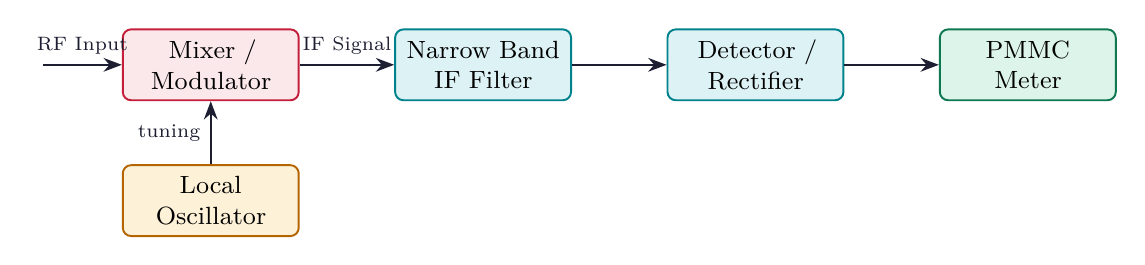
\begin{tikzpicture}[node distance=0.6cm and 1.2cm, thick, font=\small,
  sblock/.style={rectangle, draw=myteal, fill=hdrteal, text width=2.0cm,
    align=center, minimum height=0.9cm, font=\small, rounded corners=3pt, line width=0.7pt},
  sred/.style={rectangle, draw=myred, fill=hdrred, text width=2.0cm,
    align=center, minimum height=0.9cm, font=\small, rounded corners=3pt, line width=0.7pt},
  samber/.style={rectangle, draw=myamber, fill=hdramber, text width=2.0cm,
    align=center, minimum height=0.9cm, font=\small, rounded corners=3pt, line width=0.7pt},
  sgreen/.style={rectangle, draw=mygreen, fill=hdrgreen, text width=2.0cm,
    align=center, minimum height=0.9cm, font=\small, rounded corners=3pt, line width=0.7pt}]

  \node[sred] (mixer) {Mixer /\\Modulator};
  \node[sblock, right=of mixer] (filter) {Narrow Band\\IF Filter};
  \node[sblock, right=of filter] (det) {Detector /\\Rectifier};
  \node[sgreen, right=of det] (meter) {PMMC\\Meter};
  \node[samber, below=0.8cm of mixer] (lo) {Local\\Oscillator};

  % Paths
  \draw[arrow] ($(mixer.west) - (1.0, 0)$) -- node[above, font=\scriptsize] {RF Input} (mixer.west);
  \draw[arrow] (mixer) -- node[above, font=\scriptsize] {IF Signal} (filter);
  \draw[arrow] (filter) -- (det);
  \draw[arrow] (det) -- (meter);
  \draw[arrow] (lo) -- node[left, font=\scriptsize] {tuning} (mixer);
\end{tikzpicture}
\tcbset{breakable}
\end{tcolorbox}

\subsection{Total Harmonic Distortion (THD)}
Distortion analyzers measure the deviation of a waveform from a perfect sinusoid. When a pure sine wave passes through a non-linear device, harmonics are generated.

\begin{tcolorbox}[formulabox, title={\textbf{Harmonic Distortion Calculations}}]
Let $V_1$ be the fundamental component amplitude, and $V_2, V_3, \dots, V_n$ be the amplitudes of the second, third, and higher order harmonics.
\begin{itemize}[leftmargin=*, itemsep=3.5pt, topsep=0pt]
  \item \textbf{Individual Harmonic Distortion ($D_n$):}
    $$D_n = \frac{V_n}{V_1} \times 100\%$$
  \item \textbf{Total Harmonic Distortion (THD):}
    $$\text{THD} = \frac{\sqrt{V_2^2 + V_3^2 + V_4^2 + \dots + V_n^2}}{V_1}$$
  \item \textbf{THD relative to Total RMS Value ($V_{\text{rms}}$):}
    $$\text{THD}_t = \frac{\sqrt{V_2^2 + V_3^2 + \dots + V_n^2}}{\sqrt{V_1^2 + V_2^2 + \dots + V_n^2}} = \frac{\sqrt{V_{\text{rms}}^2 - V_1^2}}{V_{\text{rms}}}$$
\end{itemize}
\end{tcolorbox}

\subsection{Spectrum Analyzers}
Unlike wave analyzers that measure one frequency component at a time, a \textbf{Spectrum Analyzer} swept-tunes across a frequency band and displays the entire frequency spectrum (amplitude vs frequency) on a screen.
- \textbf{Working:} A saw-tooth sweep generator sweeps the tuning voltage of a Voltage Controlled Oscillator (VCO). This VCO serves as the local oscillator for a superheterodyne mixer, sweeping the input signal past a narrow bandpass filter. The output is rectified and drives the vertical deflection of a CRT, while the saw-tooth generator drives the horizontal sweep, yielding the spectral display.

% ===============================================================================
\section{Signal Generators}
% ===============================================================================

Signal generators produce controlled electrical waveforms for testing, calibration, and troubleshooting.

\subsection{Function Generators}
A \textbf{Function Generator} produces multiple standard waveforms (sine, square, triangular) over a wide frequency range.
- \textbf{Working Principle:} It utilizes an \textbf{integrator} and a \textbf{comparator (Schmitt trigger)} feed-back loop. The integrator charges/discharges a capacitor using constant current sources, yielding a linear triangular wave. The comparator toggles its output state at peak voltages, yielding a square wave. The triangular wave is fed through a diode-resistance wave-shaping network to approximate a low-distortion sine wave.

\subsection{Arbitrary Waveform Generators (AWG)}
An \textbf{AWG} generates custom, user-defined waveforms. It functions digitally:
1. The user defines the waveform shape mathematically or via sampling, storing the digital coordinates in a \textbf{Waveform Memory}.
2. A \textbf{Sampling Clock} drives an address counter to read out the digital words sequentially.
3. A high-speed \textbf{Digital-to-Analog Converter (DAC)} converts the digital words back into a continuous analog voltage.
4. A \textbf{Reconstruction Filter} smooths out the quantization steps.

\newpage
% ===============================================================================
% MANDATORY QUICK REVISION PAGE
% ===============================================================================
\begin{center}
  {\large\bfseries\color{myred} Quick Revision --- Module 2}\\[3pt]
  {\small\color{mydark} Signal Analyzers \& Generators $|$ OE-EC604A}
\end{center}
\noindent{\color{myred}\rule{\linewidth}{1.2pt}}
\vspace{4pt}

\begin{tcolorbox}[formulabox, title={\textbf{Key Distortion Formula}}]
$$\text{THD} = \frac{\sqrt{V_2^2 + V_3^2 + \dots + V_n^2}}{V_1} \qquad D_n = \frac{V_n}{V_1}$$
$$\text{Total AC Power RMS:} \quad V_{\text{rms}} = \sqrt{V_1^2 + V_2^2 + V_3^2 + \dots}$$
\end{tcolorbox}

\begin{tcolorbox}[defbox, title={\textbf{One-Line Definitions}}]
\begin{itemize}[leftmargin=*, itemsep=2.5pt, topsep=0pt]
  \item \textbf{Wave Analyzer:} Frequency-selective voltmeter tuned to measure a single harmonic component.
  \item \textbf{Spectrum Analyzer:} Swept-frequency instrument displaying amplitude vs frequency across a band.
  \item \textbf{THD:} Total Harmonic Distortion; ratio of root-sum-square of all harmonics to fundamental amplitude.
  \item \textbf{Function Generator:} Signal source using integrator-comparator loops to yield sine, square, and triangle waves.
  \item \textbf{Sweep Generator:} Generator sweeping output frequency automatically across a range for response plotting.
  \item \textbf{AWG:} Arbitrary Waveform Generator; digitally synthesises arbitrary user-defined waveforms from RAM.
\end{itemize}
\end{tcolorbox}

\begin{tcolorbox}[exambox, title={\textbf{Frequently Asked / Viva Questions}}]
\begin{enumerate}[topsep=0pt, label=\textbf{Q\arabic*.}, itemsep=5pt]
  \item \Q{Compare Wave Analyzers and Spectrum Analyzers.}
    A wave analyzer is a narrow-band selective voltmeter tuned manually to measure a single isolated frequency component. A spectrum analyzer automatically sweeps across a band of frequencies and displays the entire spectrum (amplitude vs frequency) in real-time.
  \item \Q{An instrument measures a fundamental component $V_1 = 10\,\text{V}$ and harmonics $V_2 = 1\,\text{V}$, $V_3 = 0.5\,\text{V}$. Calculate the THD.}\\
    Harmonic RMS: $V_h = \sqrt{V_2^2 + V_3^2} = \sqrt{1^2 + 0.5^2} = \sqrt{1 + 0.25} = \sqrt{1.25} \approx 1.118\,\text{V}$.\par
    $\text{THD} = V_h / V_1 = 1.118 / 10 = 0.1118 \implies 11.18\%$.
  \item \Q{Explain the working principle of a basic Function Generator.}
    A function generator uses an integrator and a Schmitt trigger comparator. The integrator generates a triangular wave by charging a capacitor with constant current. The comparator detects the peaks and switches the charging current direction, generating a square wave. A diode shaping network converts the triangle wave to a sine wave.
  \item \Q{What is the role of the reconstruction filter in an Arbitrary Waveform Generator (AWG)?}
    The digital-to-analog converter (DAC) reads discrete memory coordinates and outputs a stair-step approximation of the waveform. The reconstruction filter acts as a low-pass filter, removing the high-frequency quantization steps to output a smooth, continuous analog signal.
  \item \Q{What is heterodyning in HF wave analyzers?}
    Heterodyning is the mixing of an input high-frequency signal ($f_s$) with a variable local oscillator frequency ($f_{lo}$) in a non-linear mixer. This translates the target frequency component to a fixed intermediate frequency ($\text{IF} = |f_{lo} - f_s|$) where it can be filtered by a high-Q bandpass filter.
  \item \Q{Explain the function of a Sweep Frequency Generator.}
    A sweep generator automatically sweeps its output frequency continuously across a defined frequency band. It is used to test the frequency response of amplifiers, filters, and RF components by synchronizing the sweep with an oscilloscope display.
  \item \Q{What is a Capacitance-Voltage (C-V) meter and what is it used for?}
    A C-V meter measures the capacitance of a semiconductor junction (e.g., diode, MOS capacitor) as a function of an applied DC bias voltage. It is used to analyze doping profiles, oxide thickness, and interface trap densities.
  \item \Q{What is harmonic distortion and what causes it?}
    Harmonic distortion is the presence of unwanted integer multiples (harmonics) of the fundamental frequency in a signal. It is caused by non-linearities in electronic components (like transistors, diodes, or saturated magnetic cores) within the signal path.
  \item \Q{How does a Spectrum Analyzer generate its horizontal scale?}
    A saw-tooth ramp generator drives both the horizontal sweep plates of the display tube and the tuning voltage input of a voltage-controlled oscillator (VCO). This ensures that the horizontal position directly corresponds to the frequency of the local oscillator.
  \item \Q{Define the term Form Factor in AC measurements.}
    Form factor is the ratio of the RMS value of a waveform to its average value ($\text{Form Factor} = V_{\text{rms}} / V_{\text{avg}}$). For a pure sine wave, it is $1.11$.
\end{enumerate}
\end{tcolorbox}

\begin{tcolorbox}[tikzbox, title={Wave Analyzer vs Spectrum Analyzer Comparison}]
\renewcommand{\arraystretch}{1.4}
\par\noindent
\begin{tabularx}{\linewidth}{|B{2.2cm}|>{\small\centering\arraybackslash}X|>{\small\centering\arraybackslash}X|}
\hline
\textbf{Parameter} & \textbf{\color{myred}Wave Analyzer} & \textbf{\color{myteal}Spectrum Analyzer} \\
\hline
\textbf{Display Mode} & Single meter deflection indicator. & Real-time CRT/LCD spectral plot. \\
\hline
\textbf{Domain} & Single isolated frequency point. & Entire selected frequency band. \\
\hline
\textbf{Sweep} & Manual tuning only. & Automatic swept-tuned VCO. \\
\hline
\textbf{Complexity} & Lower, behaves as a narrow tuner. & High, requires VCO and sweep generator. \\
\hline
\end{tabularx}
\end{tcolorbox}

\end{document}
